\section{Fundamento técnico-conceptual}

\subsection{Análisis de mercado}
Se realiza un periodo de investigación donde se recopilan modelos ya existentes en el mercado actual para solventar la problemática proporcionada.


\subsubsection{GrabCAD}
GrabCAD es una plataforma comunitaria donde ingenieros y diseñadores comparten modelos 3D, ensamblajes y recursos CAD.\@ Permite subir, buscar, previsualizar y descargar modelos en formatos comunes (p.\,ej.\ STEP/IGES, STL, SLDPRT), organizar colecciones y discutir mejoras en comentarios. Suele incluir descripciones, imágenes renderizadas y, en algunos casos, archivos auxiliares (planos o BOM).

\newpage

\subsection{Inspiraciones}

\begin{multicols}{2}
% images

\begin{figure}[H]
  \centering
  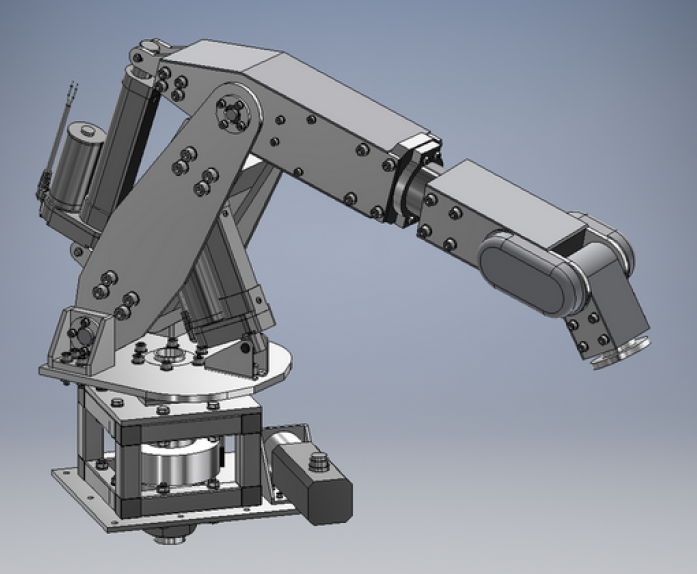
\includegraphics[width=0.4\textwidth]{anexos/inspiraciones/1actuadores.png}
  \caption{Modelo con actuadores lineales~\cite{grabcad_robot_arm_6dof}.}\label{fig:insp.actuadores}
\end{figure}

Inspiración inicial tomada de GrabCAD para un modelo con actuadores actuadores lineales. Se observa como se posicionarían los actuadores dentro del modelo para lograr una mejor distribución de masa.

\begin{figure}[H]
  \centering
  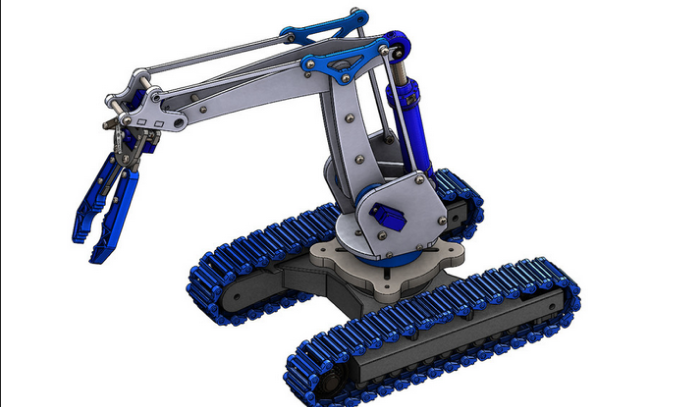
\includegraphics[width=0.4\textwidth]{anexos/inspiraciones/2oruga.png}
  \caption{Modelo hibrido/hidráulico~\cite{grabcad_robotic_arm_216}.}\label{fig:insp.oruga}
\end{figure}

Modelo mixto con servomotores y actuadores lineales encontrado en GrabCAD, primera consideración para el uso de eslabones y articulaciones. En este modelo se aprecia la restricción del movimiento de la acticulación final del manipulador.

\begin{figure}[H]
  \centering
  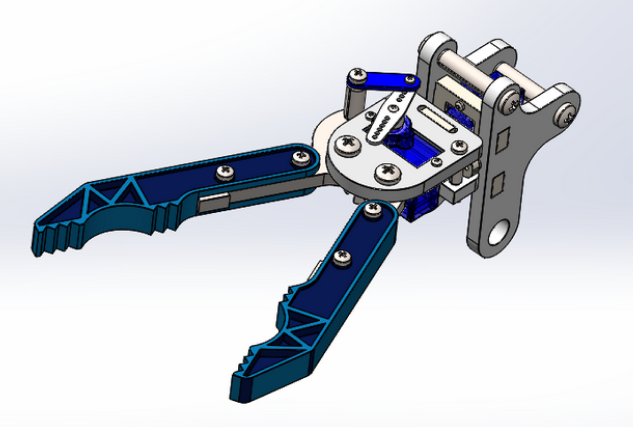
\includegraphics[width=0.4\textwidth]{anexos/inspiraciones/3orugaGarra.png}
  \caption{Manipulador por garra y servomotor~\cite{grabcad_robotic_gripper_17}.}\label{fig:insp.orugaGarra}
\end{figure}

Modelo aparte del manipulador con el servomotor sg90 y la garra. A partir de este modelo se considera el uso de un servomotor más pequeño para aprovechar que el manipulador no requiere tanta fuerza de agarre y delegar los servomotores más potentes mg996r a realizar el movimiento de las articulaciones. 

\begin{figure}[H]
  \centering
  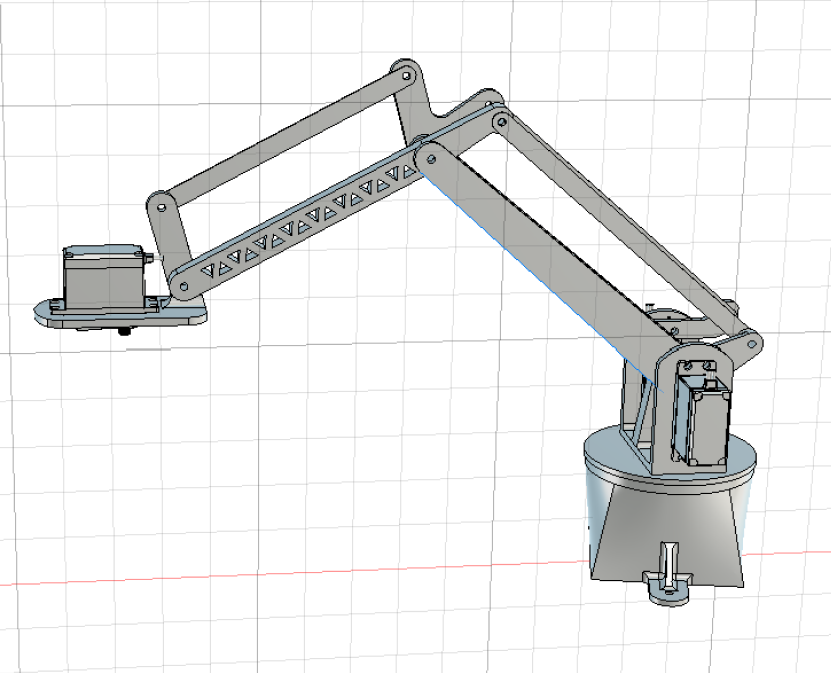
\includegraphics[width=0.4\textwidth]{anexos/inspiraciones/4eslabones.png}
  \caption{Sistema de eslabones~\cite{grabcad_sea_reach_robot_arm}.}\label{fig:insp.eslabones}
\end{figure}

Otra inspiración para implementar el uso de eslabones en el brazo robótico ya con el uso de servomotores mg996r (encontrado en GrabCAD)

\begin{figure}[H]
  \centering
  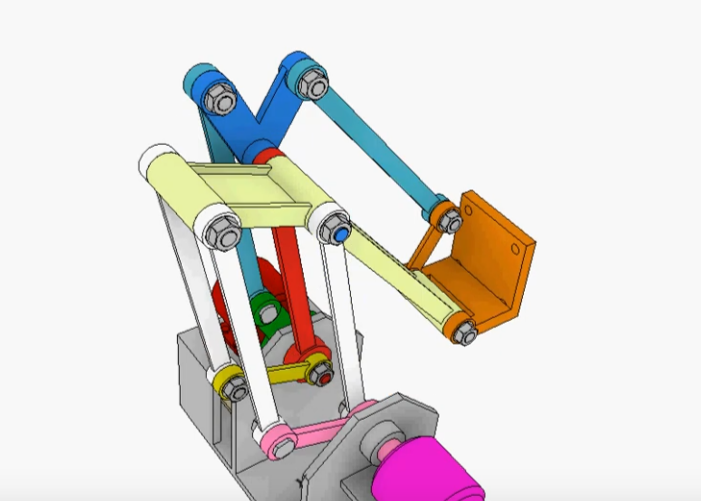
\includegraphics[width=0.4\textwidth]{anexos/inspiraciones/5eslabones.png}
  \caption{Sistema de eslabones con mayor libertad~\cite{youtube_robot_arm_link}.}\label{fig:insp.eslabones2}
\end{figure}

Una idea más general del posicionamiento de los eslabones porporcionado por el creador de contenido `thang010146' en YouTube. Este modeo cuenta con el grado de libertad faltante en modelos anteriores

\begin{figure}[H]
  \centering
  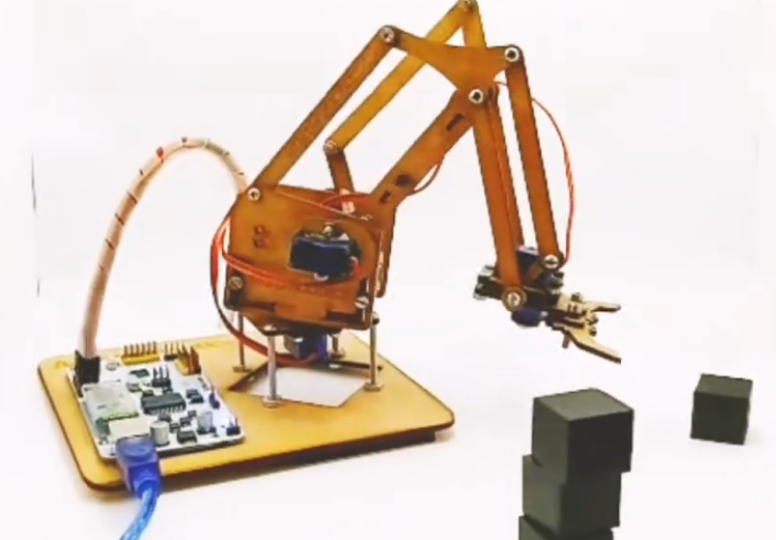
\includegraphics[width=0.4\textwidth]{anexos/inspiraciones/6mdf.png}
  \caption{Modelo en MDF~\cite{youtube_robot_arm_mdf}.}\label{fig:insp.mdf}
\end{figure}

Implemetación de un brazo robótico con especificaciones similares a las buscadas y haciendo uso de materiales como MDF y tornillos. Se descubre que el modelo pertenece a una empresa Mejicana llamada Robodacta, y que distribuyen este brazo como un kit de aprendizaje ensamblable.

\begin{figure}[H]
  \centering
  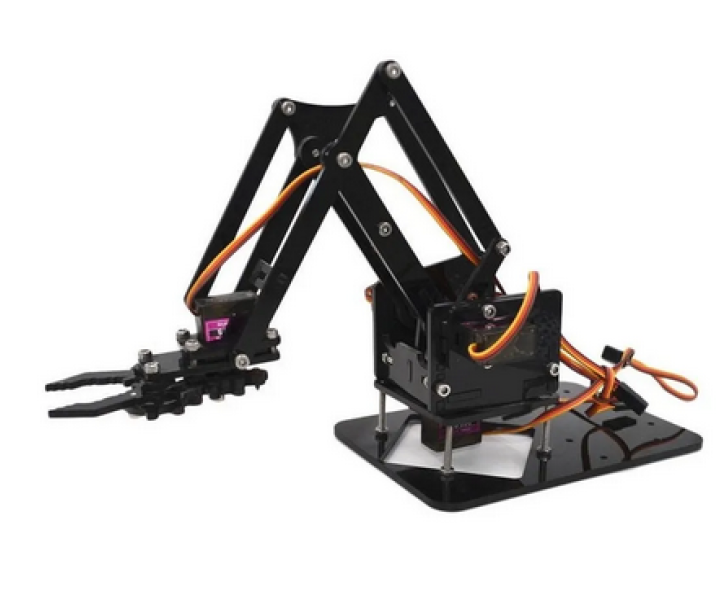
\includegraphics[width=0.4\textwidth]{anexos/inspiraciones/7plastico.png}
  \caption{Modelo similar en plástico~\cite{mercadolibre_robot_arm}.}\label{fig:insp.plastico}
\end{figure}

Modelo muy similar al anterior, haciendo uso de materiales plásticos y tornillos, comercializado en Uruguay por Mercado Libre.

\begin{figure}[H]
  \centering
  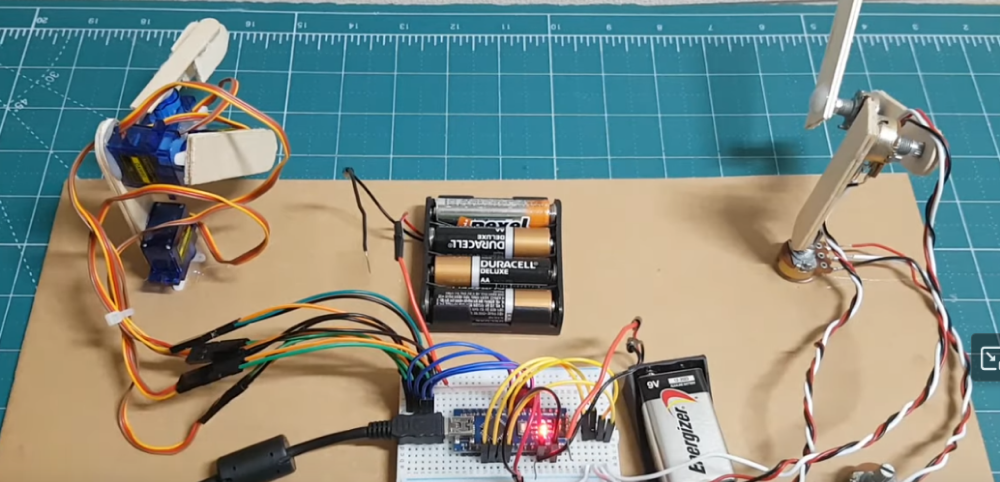
\includegraphics[width=0.4\textwidth]{anexos/inspiraciones/8control.png}
  \caption{Controlador espejo con potenciometros~\cite{youtube_robot_arm_control}}\label{fig:insp.control}
\end{figure}
Inspiración dedicada a la realización de un control `espejo' para comandar el brazo articulado, haciendo usod e potenciometros los cuales controlan el ángulo de cada articulación.

\begin{figure}[H]
  \centering
  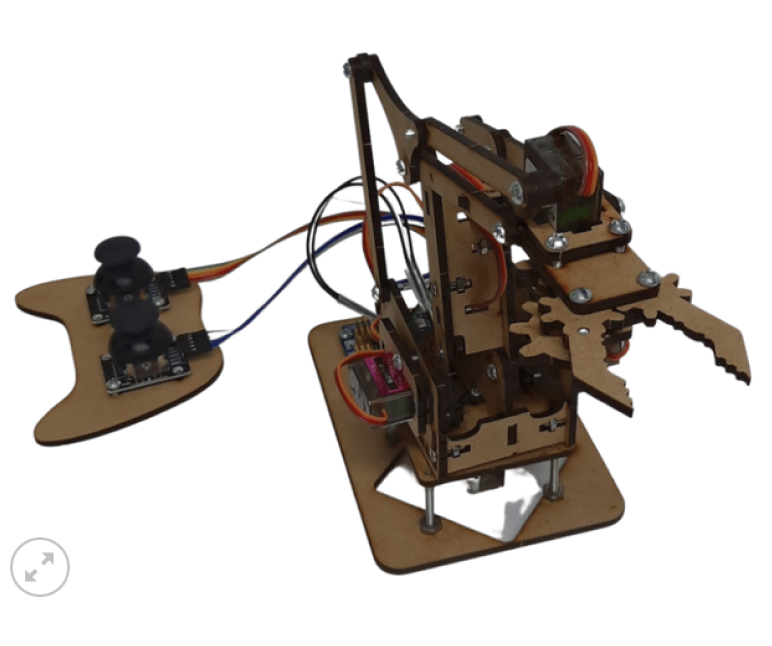
\includegraphics[width=0.4\textwidth]{anexos/inspiraciones/9joystick.png}
  \caption{Control por joystick~\cite{robodacta_mini_arm_joystick}}\label{fig:insp.joystick}
\end{figure}

Modelo original de Robodacta, el cual se encuentra publicado en su sitio web. Este cuenta con un control de joystick para comandar el brazo articulado.

\begin{figure}[H]
  \centering
  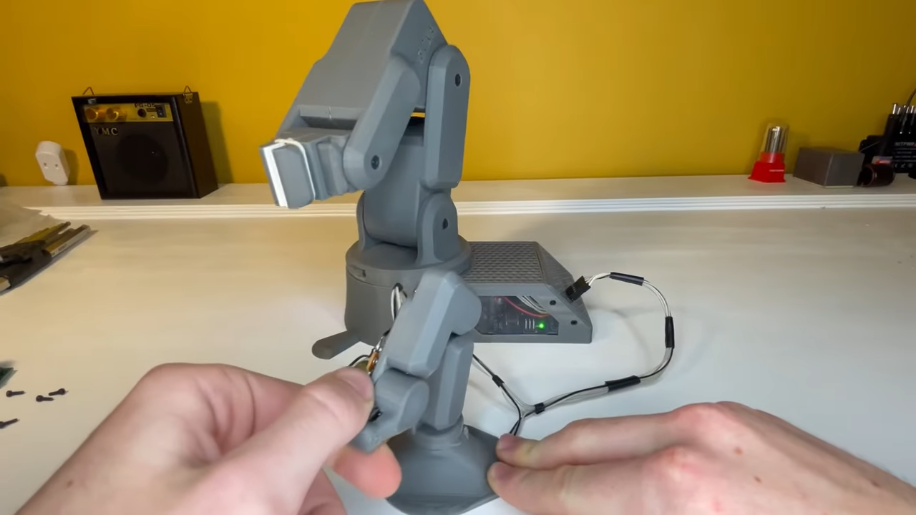
\includegraphics[width=0.4\textwidth]{anexos/inspiraciones/10impreso.png}
  \caption{Modelo impreso con control espejo~\cite{youtube_robot_arm_mirror}}\label{fig:insp.impreso}
\end{figure}

Modelo impreso de código libre por el creador de contenido `Build Some Stuff' con un sistema de control espejo similar al mostrado anteriormente. Dispone de una serie de videos mostrando materiales, ensamblaje, software y uso del brazo articulado con su controlador. Muestra funcionalidades similares a las que se pretende implementar en el proyecto.

\end{multicols}

\subsection{Diseños considerados}
Todas las soluciones involucran un brazo robótico de 4 articulaciones controladas por un Arduino. Las variaciones en los modelos se pueden clasificar en como se manejan las articulaciones y los actuadores utilizados. Las clasificaciones son:

\begin{itemize}
  \item \textbf{Servomotores MG996R.} Un modelado directo y más convencional del brazo robótico, utilizando un servomotor por articulación y colocado directamente en la misma. Apuntando el diseño a la simplicidad, en fácil ensamblado y la reparabilidad, utilizando una combinación entre corte láser en de mdf (en mayor medida) e impresión 3d.
  
  \item \textbf{Servomotores MG996R con eslabones.} Modelo implementado con servomotores pero optimizando la distribución de peso alojando a los mismos lo más cerca del eje de rotación de cada articulación y transmitiendo el movimiento mediante eslabones y palancas, buscando mejorar la eficiencia mecánica. El diseño se vuelve más vistoso y potencialmente útil para instruir en el uso de eslabones y mecanismos simples, sin embargo aumenta la complejidad del diseño llevando mayor cantidad de partes móviles, y disminuyendo la facilidad de ensamble y reparación.

  \item \textbf{Actuadores lineales tornillo---tuerca (motor DC con reductora).} Ofrecen alta fuerza y buen costo por actuador, y pueden estar enfocados a niveles educativos superiores por la implementación de controles PID con sensado de ángulo y calibración manual, entre otras cosas. Sin embargo, el mecanismo es más lento y menos preciso; requiere encoders o potenciómetros y finales de carrera para conocer el ángulo articular. Además, el diseño de eslabones y articulaciones se torna más complejo,  y los mecanismos de codificación de posición son más propensos a \emph{interferencias/ruido} y se convierten en otro posible punto de fallo. El juego mecánico (backlash) y la fricción, además del desgaste de los potenciometros pueden degradar la repetibilidad.

  \item \textbf{Actuadores lineales con asistencia hidráulica (jeringas).} Siendo la alternativa más atractiva, pero también la más compleja. Añade una capa de transmisión hidráulica sobre el actuador lineal. A cambio, ofrece una \emph{relación fuerza---peso} muy favorable (bajo peso en el extremo móvil frente a la fuerza aplicable). No obstante, introduce menor velocidad, necesidad de purgado/cebado, riesgo de fugas y mayor mantenimiento; el control (válvulas, amortiguación) eleva la complejidad significativamente. Al igual que en la opción de tornillo---tuerca, la posición debe codificarse (p.\,ej., potenciómetros/encoders lineales), añadiendo potenciales puntos de fallo.
\end{itemize}


\begin{table}[H]
\centering
\begin{tabular}{l c c c c}
\toprule
\textbf{Criterio} & \textbf{Peso} & \textbf{Servo} & \textbf{Actuador} & \textbf{Hidráulico} \\
\midrule
Peso        & 0.10 & 4 & 3 & 3 \\
Velocidad   & 0.20 & 4 & 2 & 1 \\
Simplicidad & 0.30 & 5 & 2 & 1 \\
Precio      & 0.20 & 4 & 4 & 4 \\
Fuerza      & 0.15 & 3 & 4 & 5 \\
Libertad    & 0.05 & 5 & 3 & 3 \\
\midrule
\textbf{Total ponderado} &       & \textbf{4.20} & \textbf{2.85} & \textbf{2.50} \\
\bottomrule
\end{tabular}
\caption{Matriz de selección de actuadores (1 = peor, 5 = mejor). Totales calculados con los pesos indicados.}
\end{table}


\subsubsection*{Decisión técnica}
Se implementa la solución con \textbf{servomotores MG996R} por simplicidad de control, velocidad adecuada y disponibilidad, manteniendo el costo dentro del objetivo y una fuerza suficiente para las tareas de \emph{pick \& place}. 
No obstante, se adopta la filosofía de diseño observada en las alternativas de actuadores lineales e hidráulicos: 
\emph{concentrar masa cerca de los ejes de rotación} y \emph{transmitir el movimiento mediante eslabones} hasta las articulaciones distales. 
Con ello se reduce el brazo de palanca efectivo sobre cada servo, disminuye el par exigido y se baja la inercia en el extremo móvil, 
conservando parte de los beneficios de aquellas soluciones sin incorporar su complejidad de sensado y control.

\paragraph{Lineamientos de diseño adoptados}
\begin{itemize}
  \item Ubicar los actuadores lo más cerca posible de los ejes principales o de la base para minimizar el par requerido.
  \item Emplear eslabones/bielas para accionar articulaciones alejadas, manteniendo baja la masa en el efector.
  \item Limitar configuraciones que generen grandes brazos de palanca y añadir topes/curvas de velocidad para proteger a los servos.
  \item Mantener la \emph{modularidad} e \emph{intercambiabilidad} del efector (electroimán/garra) y el diseño paramétrico para distintos espesores de MDF.\@
\end{itemize}

En síntesis, el resultado es un diseño híbrido control directo con servos potentes y una arquitectura mecánica inspirada en sistemas lineales/hidráulicos que traslada masa hacia la estructura fija. 
Esto simplifica la implementación y el mantenimiento, a la vez que mejora la eficiencia mecánica y la repetibilidad del prototipo.

\newpage

\section{Alcance}

\subsection{Alcance del proyecto}
El proyecto comprende el diseño, construcción y validación de un brazo robótico didáctico a escala. La arquitectura mecánica contempla cuatro grados de libertad (sin contar el efector), con una estructura paramétrica diseñada para corte láser en MDF de espesores entre 3.2 y 10 mm, pero adaptable también a materiales como acrílico o metal. La base será fija y deberá estar contenida dentro de un volumen de 50 $\times$ 50 $\times$ 50 cm.

El sistema contará con efectores intercambiables, entre ellos un electroimán para la manipulación de piezas ferromagnéticas y una garra mecánica para piezas no magnéticas. Ambos estarán diseñados con un mecanismo de cambio rápido que permita alternar entre uno y otro sin dificultad.

La actuación del brazo se logrará mediante servomotores MG996R, con uno por cada articulación principal. Para optimizar el rendimiento, se implementará una transmisión por eslabones que mantenga la mayor parte de la masa cercana a los ejes de giro.

En cuanto al control y la electrónica, se utilizará un microcontrolador (ESP32 o ATmega328P), un driver MOSFET como el IRFZ44N (o equivalente) para gobernar el electroimán, así como finales de carrera para homing y elementos de señalización visual y sonora mediante LEDs y un buzzer de estado.

El software incluirá un firmware desarrollado en C/C++ y una interfaz gráfica en Python, implementada en Tkinter o PyQt. Esta ofrecerá un modo manual y un modo automático, además de control ON/OFF del electroimán y una cinemática inversa planar básica para la manipulación de piezas.

La alimentación del sistema se resolverá con una fuente capaz de abastecer tanto la lógica como la potencia, incorporando convertidores adecuados para los servos y el electroimán.

Finalmente, en el componente de documentación y docencia, se elaborará un manual de armado, una guía docente y un conjunto mínimo de cinco prácticas de laboratorio orientadas a la enseñanza y experimentación con el brazo robótico.


\subsection{Fuera de alcance}
Se considera fuera de alcanze una versión implementada con actuadores lineales o hidráulicos (solo se documentan como alternativas). Además, incorporar algún tipo de visión artificial o seguimiento por cámara con planificación avanzada de trayectorias en 3D. Finalmente, se considera fuera de alcance la calibración metrológica de alta precisión o certificaciones industriales.


\subsection{Criterios de aceptación}
El dispositivo debe ser capaz de ejecutar trayectorias punto a punto tanto en modo manual como en modo automático. Asimismo, deberá alcanzar una tasa de éxito superior al 90 \% en las tareas de agarre y manipulación de objetos, garantizando un desempeño confiable durante su operación.

De igual forma, contará con una rutina de referencia operativa que asegure la correcta inicialización del sistema, un mecanismo de paro de emergencia y límites mecánicos verificados para preservar la seguridad del equipo y del entorno.

Finalmente, el proyecto se entregará con un prototipo completamente ensamblado, acompañado del firmware correspondiente, la interfaz gráfica de usuario, un manual de usuario detallado y una guía docente que incluya cinco prácticas evaluables para su aplicación en el ámbito académico.
